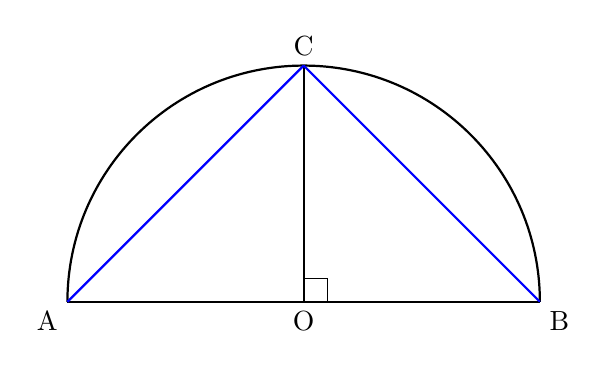
\begin{tikzpicture}
    % Draw the semicircle centered at O
    \draw[thick] (-3,0) arc[start angle=180, end angle=0, radius=3cm];
    
    % Draw the radius lines OA and OB
    \draw[thick] (0,0) -- (3,0);
    \draw[thick] (0,0) -- (-3,0);
    
    % Draw the line segments from O to C and from A and B to C
    \draw[thick] (0,0) -- (0,3);
    \draw[thick, blue] (0,3) -- (3,0);
    \draw[thick, blue] (0,3) -- (-3,0);
    
    % Label points A, B, C, and O
    \node[below left] at (-3,0) {A};
    \node[below right] at (3,0) {B};
    \node[above] at (0,3) {C};
    \node[below] at (0,0) {O};
    
    % Right angle marker at O
    \draw (0,0) -- (0.3,0) -- (0.3,0.3) -- (0,0.3) -- cycle;
\end{tikzpicture}

